%\documentclass[10pt, conference, letterpaper]{IEEEtran}
%%\documentclass[10 pt, conference]{ieeeconf}
%%\documentclass[letterpaper, 10 pt, conference]{ieeeconf}
%\documentclass[12pt,draftcls,peerreviewca,onecolumn,a4paper,dvips]{IEEEtran}


\documentclass[12pt,onecolumn]{IEEEtran}
%\documentclass[10pt,conference]{IEEEtran}


%*************prof with Delta t************


%\documentclass[conference]{IEEEtran}
%% INFOCOM 2013 addition:
\usepackage{etoolbox}
\makeatletter
\def\ps@headings{%
	\def\@oddhead{\mbox{}\scriptsize\rightmark \hfil \thepage}%
	\def\@evenhead{\scriptsize\thepage \hfil \leftmark\mbox{}}%
	\def\@oddfoot{}%
	\def\@evenfoot{}}
\makeatother
\pagestyle{headings}

\hyphenation{op-tical net-works semi-conduc-tor}

\usepackage{verbatim}
\usepackage{xcolor}
\usepackage{amsfonts}
\usepackage{mathrsfs}
\usepackage{amsfonts}
\usepackage{amssymb}
\usepackage{graphicx}
\usepackage{epsfig}
\usepackage{epstopdf}
\usepackage{psfrag}
\usepackage{amsmath}
\usepackage{array}
\usepackage{cases}
%\usepackage{algorithm2e}
\usepackage{subfigure}
\usepackage{cite,graphicx,amsmath,amssymb,color}
%\usepackage{amsthm}
%\usepackage{anysize}
\usepackage{algorithmic}
\usepackage{algorithm}

%from Kuan
\usepackage{algorithm}
\usepackage{algorithmic}
%\usepackage{mathbbold}
\usepackage{stmaryrd}
\usepackage{multirow}
\usepackage{subfig}
\usepackage{graphicx,times,amsmath} % Add all your packages here
\DeclareMathOperator*{\argmax}{argmax}

\usepackage{url}
\usepackage{enumerate}
%\usepackage{amsthm}

%\marginsize{left}{right}{top}{bottom}:
%\marginsize{13mm}{13mm}{19mm}{43mm}

\renewcommand{\algorithmicrequire}{ \textbf{Input:}}      %Use Input in the format of Algorithm
\renewcommand{\algorithmicensure}{ \textbf{Output:}}     %UseOutput in the format of Algorithm



\IEEEoverridecommandlockouts

\newtheorem{theorem}{Theorem}
\newtheorem{lemma}{Lemma}
\newtheorem{Cor}{Corollary}
\newtheorem{Def}{Definition}
\newtheorem{Exam}{Example}
\newtheorem{Alg}{Algorithm}
\newtheorem{Sch}{Scheme}
\newtheorem{problem}{Problem}
\newtheorem{remark}{Remark}
\newtheorem{Proof}{Proof}
\newtheorem{Asump}{Assumption}
\newtheorem{Subp}{Subproblem}
\newtheorem{case}{Case}




\begin{document}
\bibliographystyle{IEEEtran}
	
\title{Homework 2}
	%\author{Junfeng Guo, \quad  Zhaozhe Song, \quad Ying Cui\\
	%Department of Electronic Engineering, Shanghai Jiao Tong University, Shanghai, P. R. China}
	

\author{Wei Xu, Student No:117034910134}
	
	
	
	
	
%Email: \{aaa, bbb, ccc\}@sjtu.edu.cn}
\maketitle
\section{Problem 1}
In machine learning, support vector machines (SVMs) are supervised learning models with associated learning algorithms that analyze data used for classification and regression analysis.  Given a set of training examples, each marked as belonging to one or the other of two categories, an SVM training algorithm builds a model that assigns new examples to one category or the other, making it a non-probabilistic binary linear classifier. An SVM model is a representation of the examples as points in space, mapped so that the examples of the separate categories are divided by a clear gap that is as wide as possible. New examples are then mapped into that same space and predicted to belong to a category based on which side of the gap they fall.
In addition to performing linear classification, SVMs can efficiently perform a non-linear classification using what is called the kernel trick, implicitly mapping their inputs into high-dimensional feature spaces.

In this question, it is a three classification problem and we adopt the one-vs-rest (ovr) strategy. It means we should train three SVM models to classify. The ovr strategy involves training a single classifier per class, with the samples of that class as positive samples and all other samples as negatives. This strategy requires the base classifiers to produce a real-valued confidence score for its decision, rather than just a class label; discrete class labels alone can lead to ambiguities, where multiple classes are predicted for a single sample. We first classify the data as follows:
\begin{figure}[H]
	\centering
	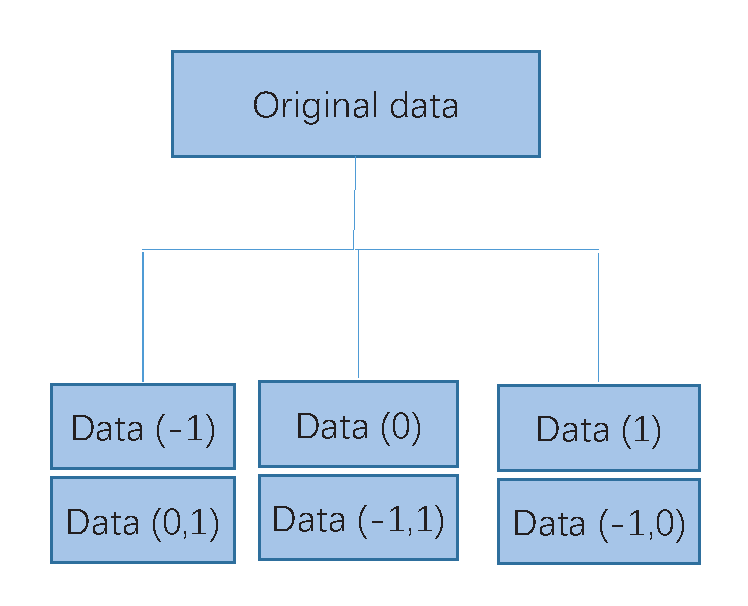
\includegraphics[width=7cm,height=5cm]{classify.eps}
	\caption{data classify}
\end{figure}


Then we use preprocessing.StandardScaler() in sklearn to standardize features by removing the mean and scaling to unit variance. This will improve the performance for SVM. We use the standard algorithm to train three SVM models. We first show the original data in 2-dimension by using dimensionality reduction.
\begin{figure}[H]
	\centering
	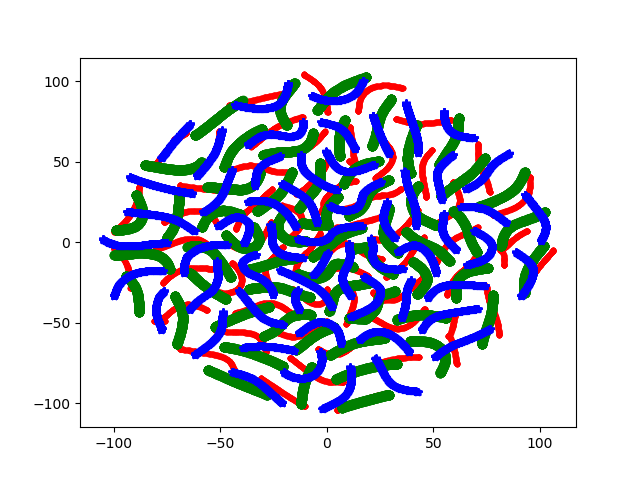
\includegraphics[width=8cm,height=7cm]{originalData.png}
	\caption{Original data after dimensionality reduction}
\end{figure}

We clearly can see after dimensionality reduction into 2-dimension, the classification is hard to solve. It seems all the data are mixed together.

After training three models, we can get the accuracy of our SVM based on ovr. Our model can get 43.5\% for this three classification problem. 

\section{Problem 2}
For the three-class classification problem, we use Min-Max-Module SVM and part-vs-part task decomposition method. We first divide the three-class problem into three two-class problems using one-vs-rest method and then decompose these imbalance two-class problems into balance two-class problems following random task decomposition.
 
In our simulation, we choose randomly 1000 sample of raw data five times and randomly choose 1000 sample of label data two times. Thus, we should train 10 SVM models and use Min-Max-Module to get the result. The scheme of Min-Max-Module can be shown as follows:
\begin{figure}[H]
\centering
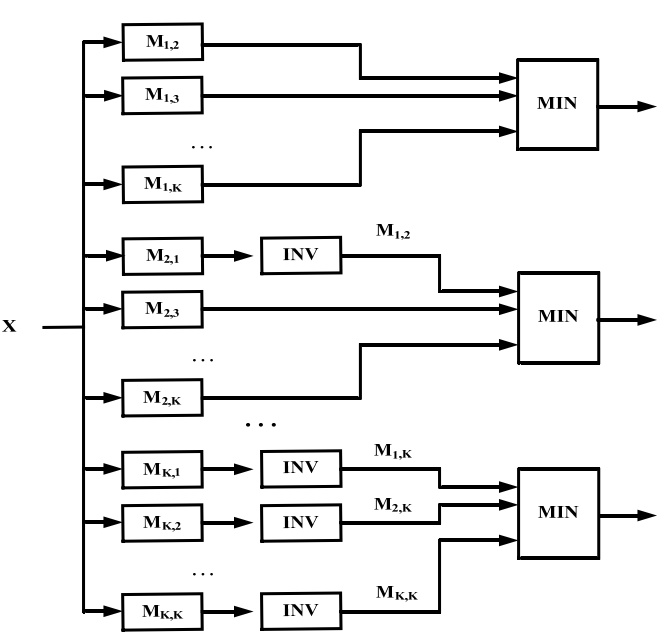
\includegraphics[width=8cm,height=8cm]{M3.png}
\caption{Min-Max-Module}
\end{figure}

After training these models, we can get the accuracy of our SVM based on part-vs-part task decomposition and Min-Max-Module. Our model can get 47.5\% for this three classification problem. Compared with Problem~1, we improve 4$\sim$5\% of accuracy. 
\end{document}